\documentclass[10pt]{article}
\usepackage[scaled=0.92]{helvet}
\usepackage{calc}
\usepackage{multicol}
\usepackage{ifthen}
\usepackage[a4paper,margin=3mm,portrait]{geometry}
\usepackage{amsmath,amsthm,amsfonts,amssymb}
\usepackage{color,graphicx,overpic}
\usepackage{hyperref}
\usepackage{newtxtext} 
\usepackage{enumitem}
\usepackage[table]{xcolor}
\usepackage{mathtools}
\setlist{nosep}

% for including images
\graphicspath{ {../images/} }

% Turn off header and footer
\pagestyle{empty}

\newenvironment{tightcenter}{%
  \setlength\topsep{0pt}
  \setlength\parskip{0pt}
  \begin{center}
}{%
  \end{center}
}

% redefine section commands to use less space
\makeatletter
\renewcommand{\section}{\@startsection{section}{1}{0mm}%
                                {-1ex plus -.5ex minus -.2ex}%
                                {0.5ex plus .2ex}%x
                                {\normalfont\large\bfseries}}
\renewcommand{\subsection}{\@startsection{subsection}{2}{0mm}%
                                {-1explus -.5ex minus -.2ex}%
                                {0.5ex plus .2ex}%
                                {\normalfont\normalsize\bfseries}}
\renewcommand{\subsubsection}{\@startsection{subsubsection}{3}{0mm}%
                                {-1ex plus -.5ex minus -.2ex}%
                                {1ex plus .2ex}%
                                {\normalfont\small\bfseries}}%
\renewcommand{\familydefault}{\sfdefault}
\renewcommand\rmdefault{\sfdefault}
%  makes nested numbering (e.g. 1.1.1, 1.1.2, etc)
\renewcommand{\labelenumii}{\theenumii}
\renewcommand{\theenumii}{\theenumi.\arabic{enumii}.}
\renewcommand\labelitemii{•}
\renewcommand\labelitemiii{•}
%  convenient absolute value symbol
\newcommand{\abs}[1]{\vert #1 \vert}
%  convenient floor and ceiling
\newcommand{\floor}[1]{\lfloor #1 \rfloor}
\newcommand{\ceil}[1]{\lceil #1 \rceil}
%  convenient modulo
\newcommand{\Mod}[1]{\ \mathrm{mod}\ #1}
%  for logical not operator, iff symbol, convenient "if/then"
\renewcommand{\lnot}{\mathord{\sim}}
\let\then\rightarrow
\let\Then\Rightarrow
%  vectors
\newcommand{\vv}[1]{\boldsymbol{#1}}
\newcommand{\VV}[1]{\overrightarrow{#1}}
%  column vector
\newcommand{\cvv}[1]{\left(\begin{smallmatrix}#1\end{smallmatrix}\right)}
\newcommand{\code}[1]{\textcolor{mygreen}{\texttt{#1}}}
\newcommand{\java}[1]{\mintinline{java}|#1|}
\newcommand\bggreen{\cellcolor{green!10}}

\makeatother
\definecolor{myblue}{cmyk}{1,.72,0,.38}
\definecolor{mygreen}{cmyk}{0.0, 0.66, 0.30, 0.33}
\everymath\expandafter{\the\everymath \color{myblue}}
% Define BibTeX command
\def\BibTeX{{\rm B\kern-.05em{\sc i\kern-.025em b}\kern-.08em
    T\kern-.1667em\lower.7ex\hbox{E}\kern-.125emX}}

% Don't print section numbers
\setcounter{secnumdepth}{0}

\setlength{\parindent}{0pt}
\setlength{\parskip}{0pt plus 0.5ex}
%% this changes all items (enumerate and itemize)
\setlength{\leftmargini}{0.5cm}
\setlength{\leftmarginii}{0.4cm}
\setlength{\leftmarginiii}{0.5cm}
\setlist[itemize,1]{leftmargin=2mm,labelindent=1mm,labelsep=1mm}
\setlist[itemize,2]{leftmargin=3mm,labelindent=1mm,labelsep=1mm}
\setlist[itemize,3]{leftmargin=3mm,labelindent=1mm,labelsep=1mm}

%My Environments
\newtheorem{example}[section]{Example}
% -----------------------------------------------------------------------

\begin{document}
\raggedright
\footnotesize
\begin{multicols}{3}


% multicol parameters
% These lengths are set only within the two main columns
\setlength{\columnseprule}{0.25pt}
\setlength{\premulticols}{1pt}
\setlength{\postmulticols}{1pt}
\setlength{\multicolsep}{1pt}
\setlength{\columnsep}{2pt}

\begin{center}
    \fbox{%
        \parbox{0.8\linewidth}{\centering \textcolor{black}{
            {\Large\textbf{CS2040S}}
            \\ \normalsize{AY23/24S2 Midterms}}
            \\ {\footnotesize Original by: \textcolor{myblue}{github.com/jovyntls}}
            \\ {\footnotesize Modified by: \textcolor{myblue}{github.com/zeepheru}}
        }%
    }
\end{center}

\section{ORDERS OF GROWTH}
\begin{tightcenter}
    $T(n) = \Theta(f(n))$
    \\* $\iff T(n) = O(f(n))$ and $T(n) = \Omega(f(n))$

    $T(n) = O(f(n))$ 
    \\* if $\exists c, n_0 > 0$ such that for all $n > n_0$, $T(n) \leq cf(n)$
    
    $T(n) = \Omega(f(n))$
    \\* if $\exists c, n_0 > 0$ such that for all $n > n_0$, $T(n) \geq cf(n)$
    
\end{tightcenter}

\subsection{properties}
Let $T(n) = O(f(n))$ and $S(n) = O(g(n))$ 
\begin{itemize}
    \item addition: $T(n) + S(n) = O(f(n) + g(n))$
    \item multiplication: $T(n) * S(n) = O(f(n) * g(n))$
    \item composition: $f_1 \circ f_2 = O(g_1 \circ g_2)$ only if both increasing
    \item if/else statements: $\text{cost} = \max(c1, c2) \leq c1+c2$
    \item max: $\max(f(n), g(n)) \leq f(n) + g(n)$
    \item $\Theta(f(n))$ time complexity $\Then O(f(n))$ space complexity
    \item space complexity: once we exit the function, release all memory that was used
\end{itemize}

% \subsubsection{notable}
% \begin{itemize}
%     \item $O(\sqrt{n}\log n) = O(n)$, $\quad O(2^{2n}) \neq O(2^n)$
%     \item $O(\log (n!)) = O(n\log n) \then$ sterling's approximation
%     \item $T(n-1) + T(n-2) + \dots + T(1) = 2T(n-1)$
% \end{itemize}

% \subsubsection{master theorem}
% $T(n) = aT(\frac{n}{b}) + f(n) \quad a \geq 0, b > 1$
% $= \begin{cases}
%     \Theta(n^{\log_ba}) & \quad \text{ if } f(n) < n^{\log_ba} \text{ polynomially}
%     \\ \Theta(n^{\log_ba} \log n) & \quad \text{ if } f(n) = n^{\log_ba} 
%     \\ \Theta(f(n)) & \quad \text{ if } f(n) > n^{\log_ba} \text{ polynomially}
% \end{cases}$

% \subsection{space complexity}
% \begin{itemize}
%     \item $\Theta(f(n))$ time complexity $\Then O(f(n))$ space complexity
%     \item max. space incurred \textbf{at any time at any point} (once we exit the function, release all memory that was used)
% \end{itemize}

\section{QUICKSORT}
\begin{itemize}
    \item stable quicksort: $O(\log n)$ space (due to recursion stack)
    \item worst case $O(n^2)$: pivot first/last/middle element
    \item worst case $O(n\log n)$: median/random element/fraction
    \item choose at random: runtime is a random variable
\end{itemize}

\section{TREES}

% \subsection{traversal}
% \begin{center}
%     \begin{multicols}{3}
%         \textit{pre-order DFS}
%         \includegraphics[width=0.9\linewidth]{../../CS1231S/images/cs1231s-ch11-preorder}
%         \\* {\tiny\textbf{F-B-A-D-C-E-G-I-H}}
        
%         \textit{in-order DFS}
%         \includegraphics[width=0.9\linewidth]{../../CS1231S/images/cs1231s-ch11-inorder}
%         \\* {\tiny\textbf{A-B-C-D-E-F-G-H-I}}
        
%         \textit{post-order DFS}
%         \includegraphics[width=0.9\linewidth]{../../CS1231S/images/cs1231s-ch11-postorder}
%         \\* {\tiny\textbf{A-C-E-D-B-H-I-G-F}}
%     \end{multicols}
% \end{center}

\subsection{AVL Trees}
\begin{itemize}
    \item \textbf{height-balanced} (maintained with rotations)
    \begin{itemize}
        \item $\iff$ \code{|v.left.height - v.right.height| $\leq 1$}
    \end{itemize}
    \item each node is augmented with its height - \code{v.height = h(v)}
    \item space complexity: $O(LN)$ for $N$ strings of length $L$
\end{itemize}

\begin{tightcenter}
    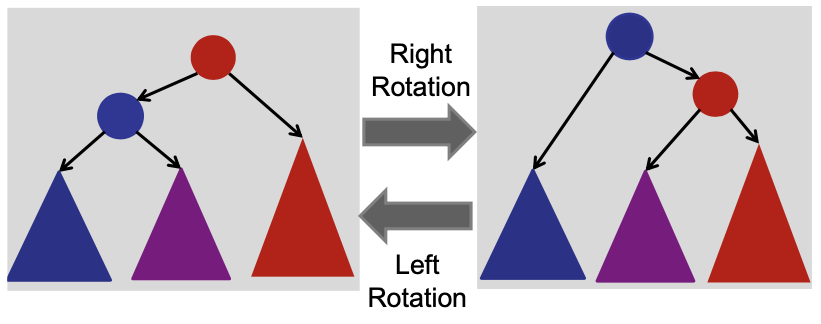
\includegraphics[width=0.8\linewidth]{cs2040s-tree-rotation.png}
    \\* \textbf{insertion} - max 2 rotations; \textbf{deletion} - recurse all the way up; 
\end{tightcenter}

\subsubsection{rebalancing}
[case 1] B is  \textbf{balanced: right-rotate}
\begin{tightcenter}
    $h(L) = h(M), \quad h(R) = h(M) - 1$
    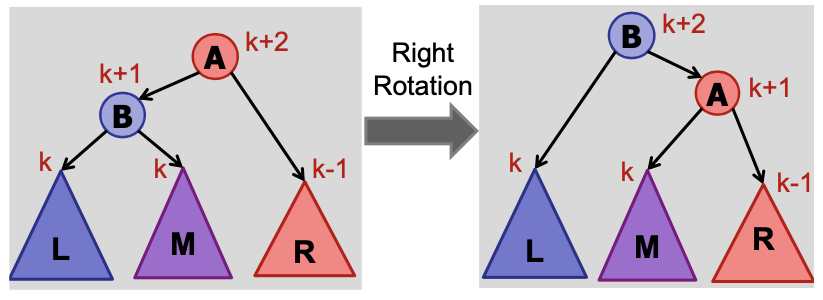
\includegraphics[width=0.65\linewidth]{cs2040s-rebalance-case-1.png}
\end{tightcenter}

[case 2] B is  \textbf{left-heavy: right-rotate}
\begin{tightcenter}
    $h(L) = h(M) + 1, \quad h(R) = h(M)$
    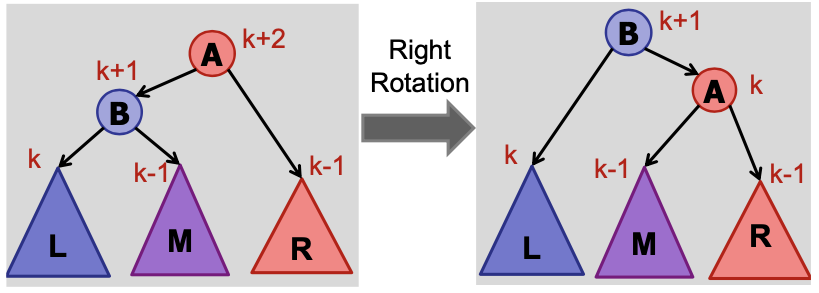
\includegraphics[width=0.65\linewidth]{cs2040s-rebalance-case-2.png}
\end{tightcenter}

[case 3] B is  \textbf{right-heavy: left-rotate(v.left), right-rotate(v)}
\begin{tightcenter}
    $h(L) = h(M) - 1, \quad h(R) = h(L)$
    \\* 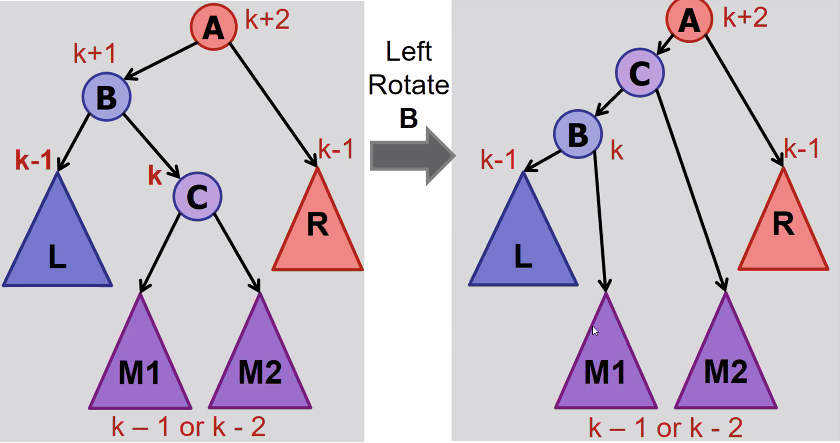
\includegraphics[width=0.65\linewidth]{cs2040s-rebalance-case-3-1.png}
    \\* 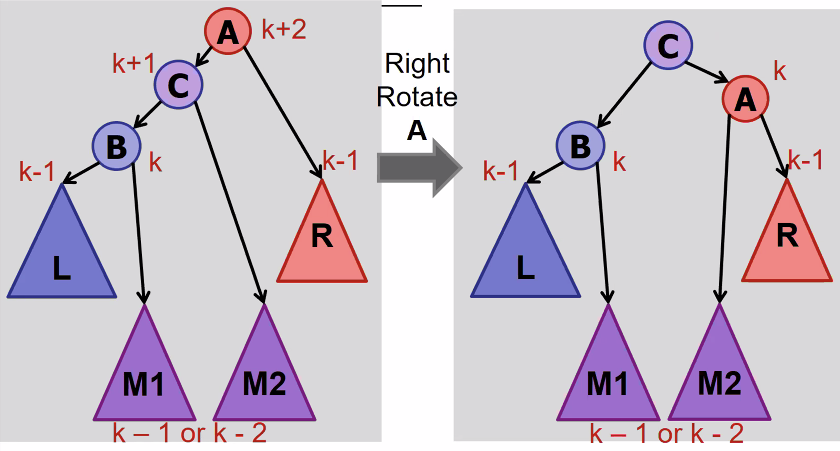
\includegraphics[width=0.65\linewidth]{cs2040s-rebalance-case-3-2.png}
\end{tightcenter}

\subsubsection{updating nodes after rotation}
\begin{tightcenter}
    weights:
    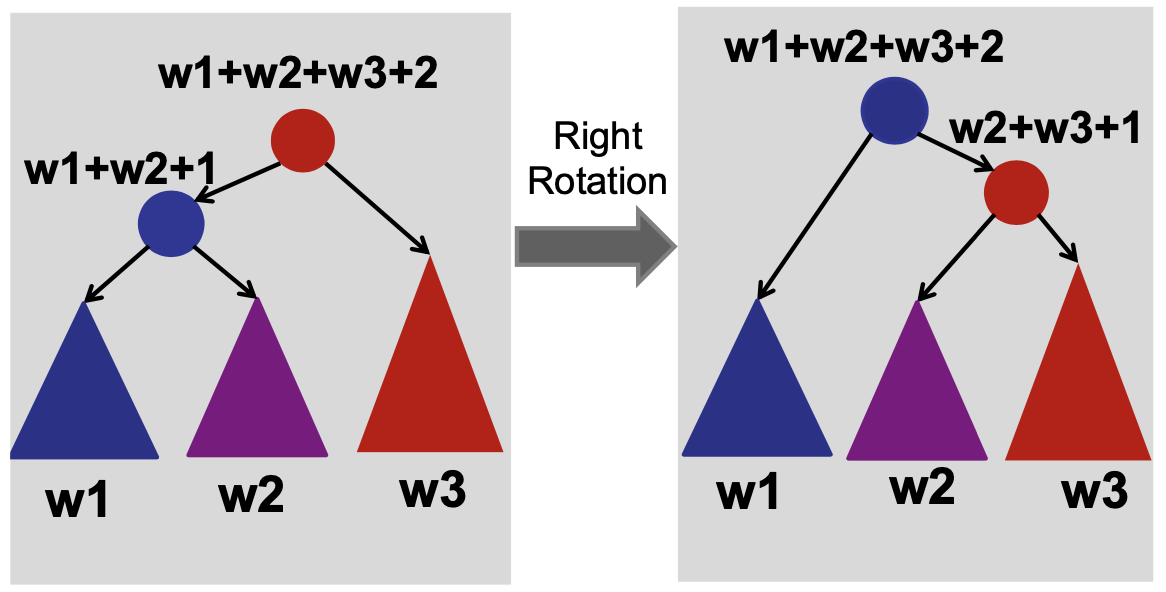
\includegraphics[width=0.65\linewidth]{cs2040s-rotate-weights.png}
    
    max:
    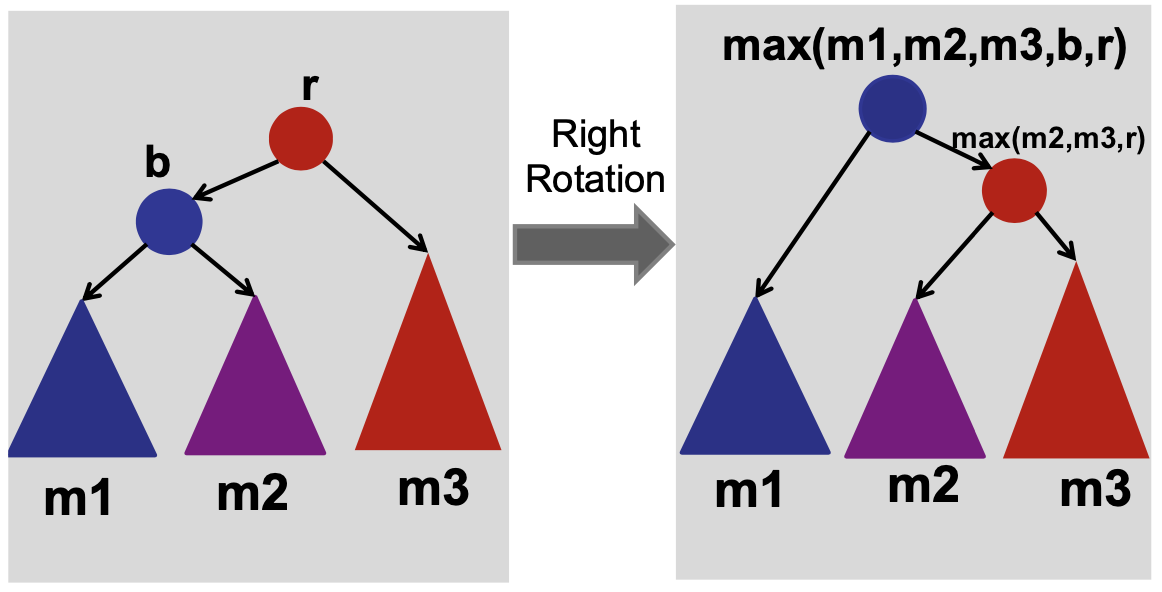
\includegraphics[width=0.65\linewidth]{cs2040s-rotate-max.png}
\end{tightcenter}

\subsection{binary search trees (BST)}
\begin{itemize}
    \item balanced: $O(h) = O(\log n)$ (depends on insertion order)
    \item for a full-binary tree of size $n, \exists k \in \mathbb{Z}^+$ s.t. $n=2^k-1$ 
    \item \code{height, h(v) = max(h(v.left), h(v.right))}
    \begin{itemize}
        \item leaf nodes: \code{h(v)} = 0 
    \end{itemize}
    \item \code{search}, \code{insert} - $O(h)$
    \item \code{delete} - $O(h)$
    \begin{itemize}
        \item no children - remove the node
        \item 1 child - remove the node, connect parent to child
        \item 2 children - delete successor; replace node w successor
    \end{itemize}
    \item \code{searchMin/Max} - $O(h)$ - recurse into left/right subtree
    \item \code{successor} - $O(h)$
    \begin{itemize}
        \item if node has a right subtree: \code{searchMin(v.right)}
        \item else: traverse upwards and return the first parent that contains the key in its left subtree
    \end{itemize}
    \item \textbf{merkle trees}
    \begin{itemize}
        \item binary tree - nodes augmented with a hash of their children
        \item same root value = identical tree
    \end{itemize}
\end{itemize}

\subsection{Trie}
\begin{itemize}
    \item \code{search, insert} - $O(L)$ (for string of length $L$)
    \item space: $O($size of text $\cdot$ overhead$)$
\end{itemize}

\subsection{interval trees}
\begin{itemize}
    \item \code{search(key)} $\Then O(\log n)$
    \begin{itemize}
        \item if value is in root interval, return
        \item if value > max(left subtree), recurse right
        \item else recurse left (go left only when can't go right)
    \end{itemize}
    \item all-overlaps $\Then O(k \log n)$ for $k$ overlapping intervals
\end{itemize}

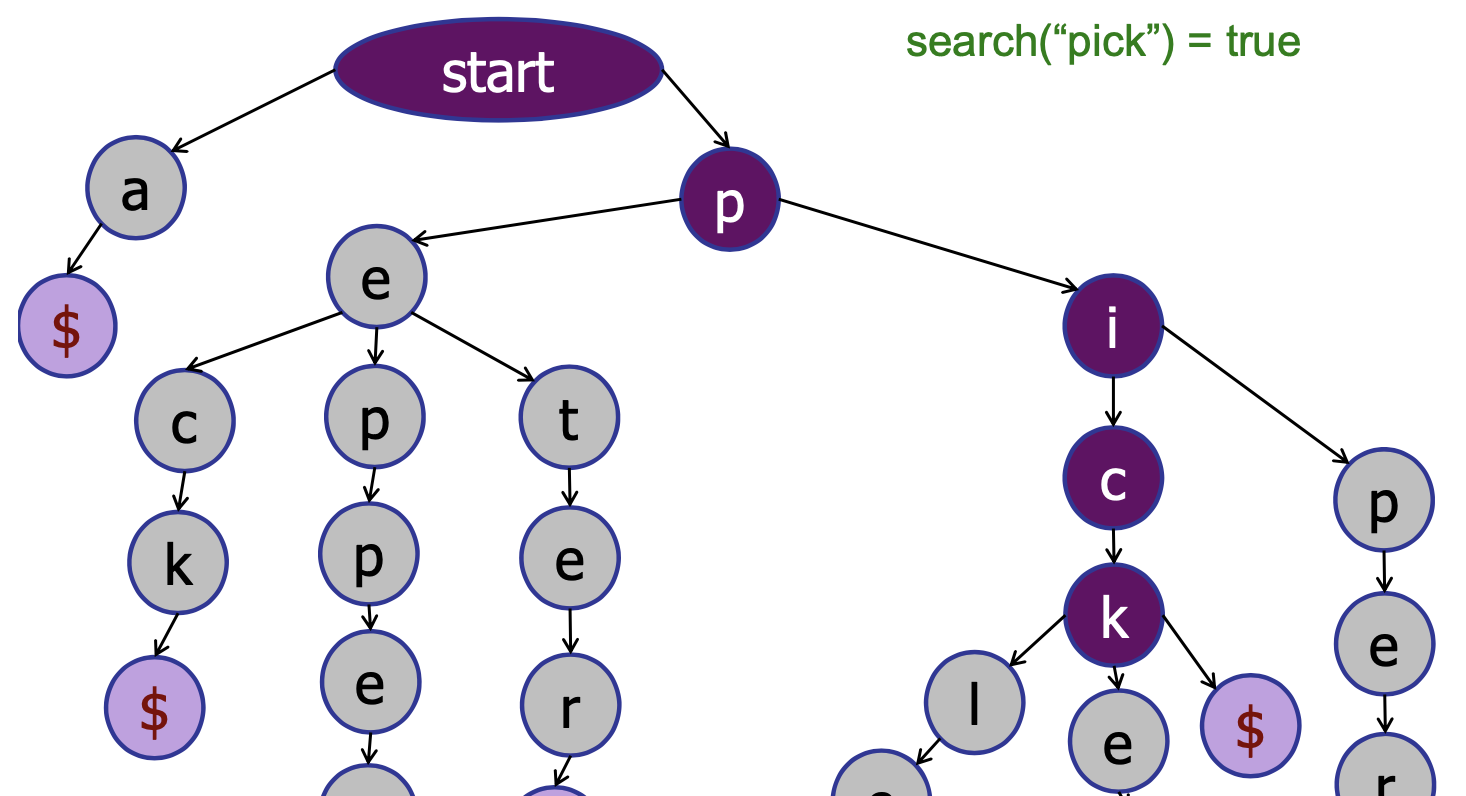
\includegraphics[width=0.5\linewidth]{cs2040s-trie.png}
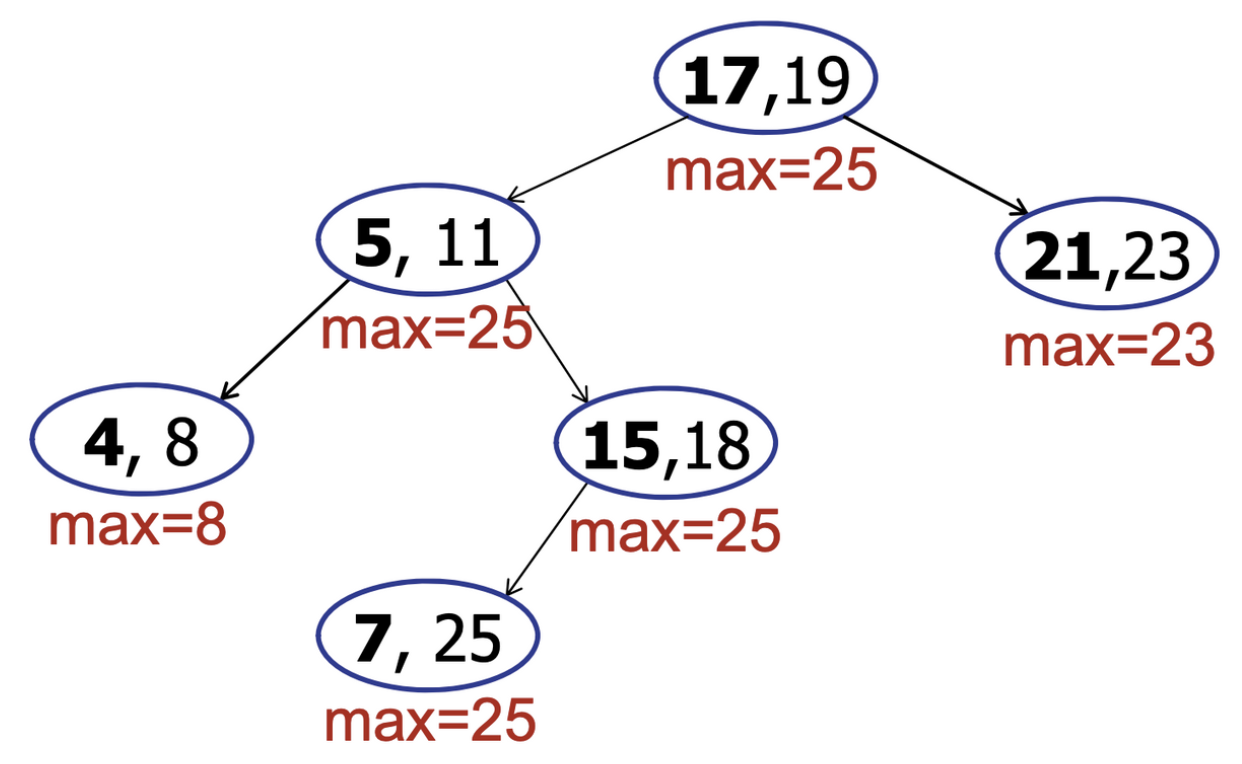
\includegraphics[width=0.45\linewidth]{cs2040s-interval-tree.png}

\subsection{orthogonal range searching}
\begin{itemize}
    \item binary tree; leaves store points, internal nodes store max value in left subtree
    \item \code{buildTree(points[])} $\Then O(n \log n)$ \quad (space is $O(n)$)
    \item \code{query(low, hight)} $\Then O(k + \log n)$ for $k$ points
    \begin{itemize}
        \item \code{v=findSplit()} $\Then O(\log n)$ - find node b/w low \& high
        \item \code{leftTraversal(v)} $\Then O(k)$ - either output all the right subtree and recurse left, or recurse right 
        \item \code{rightTraversal(v)} - symmetric
    \end{itemize}
    \item \code{insert(key), insert(key)} $\Then O(\log n)$ 
    \item \code{2D\_query()} $\Then O(\log^2n + k)$ \quad (space is $O(n \log n)$)
    \begin{itemize}
        \item build x-tree from x-coordinates; for each node, build a y-tree from y-coordinates of subtree
    \end{itemize}
    \item \code{2D\_buildTree(points[])} $\Then O(n \log n)$
\end{itemize}

\subsection{kd-Tree}
\begin{itemize}
    \item stores geometric data (points in an $(x, y)$ plane)
    \item alternates splitting (partitioning) via $x$ and $y$ coordinates
\end{itemize}
\begin{minipage}{0.4\linewidth}   
    \begin{tightcenter}
        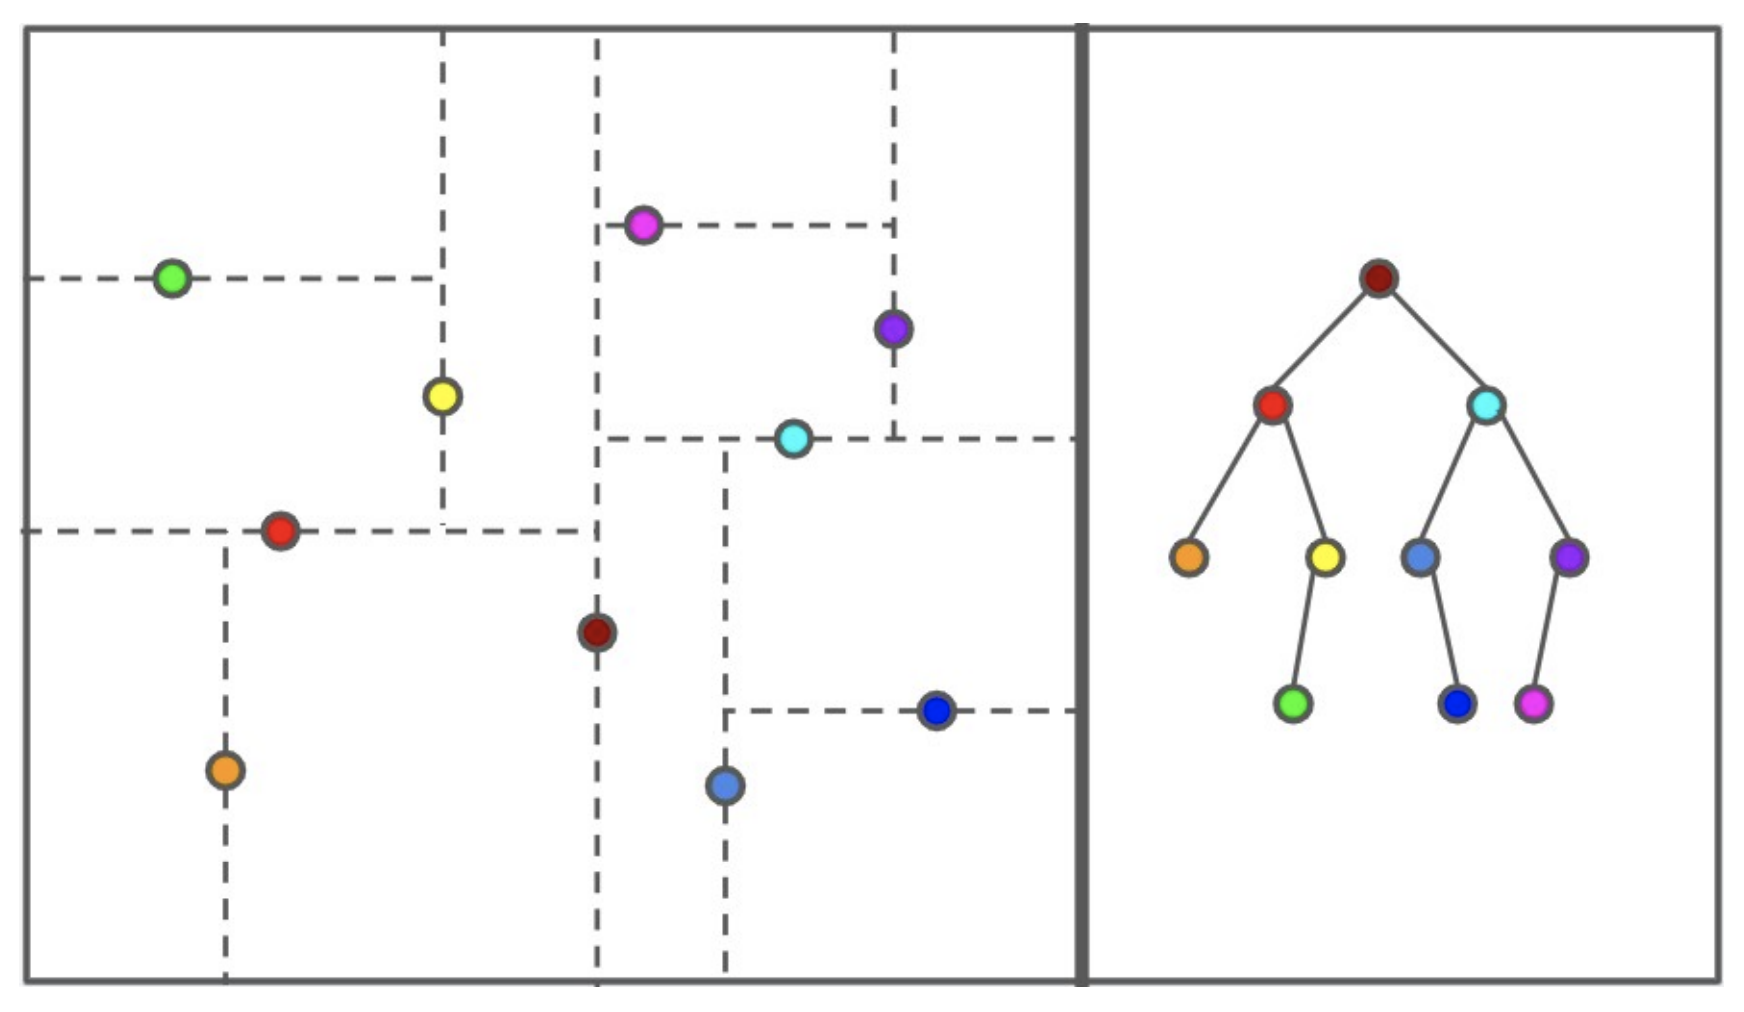
\includegraphics[width=0.95\linewidth]{cs2040s-kdtree.png}
    \end{tightcenter}
\end{minipage}
\begin{minipage}{0.55\linewidth}
    \begin{itemize}
        \item \code{construct(points[])} 
            \\* $\Then O(n \log n)$
        \item \code{search(point)} $\Then O(h)$
        \item \code{searchMin()} $\Then O(\sqrt{n})$
            \\* $\Then T(n) = 2T(\frac{n}{4}) + O(1)$
    \end{itemize}
\end{minipage}



\subsection{(a, b)-trees}
{\scriptsize{e.g. a (2, 4)-tree storing 18 keys}}
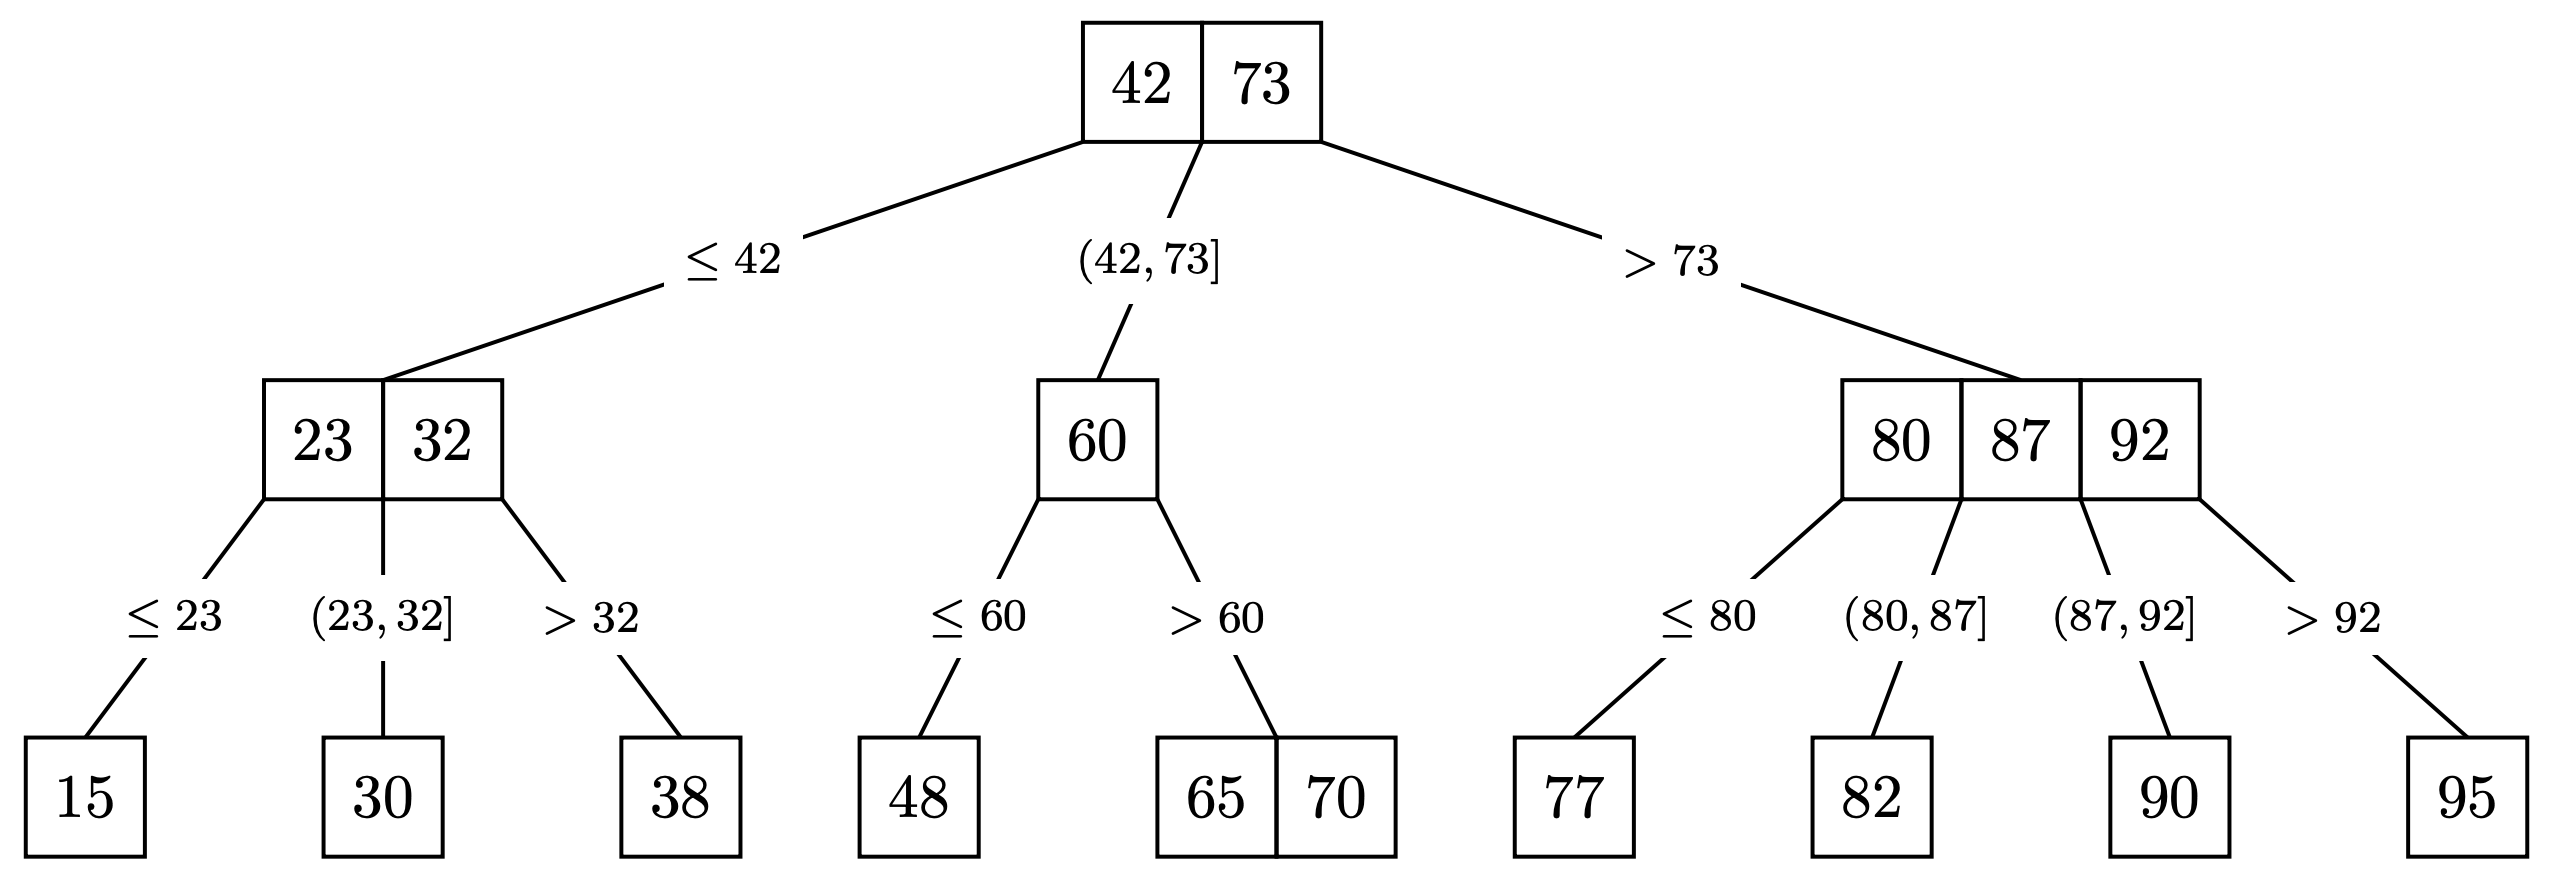
\includegraphics[width=0.8\linewidth]{cs2040s-ab-tree.png}
\begin{itemize}
    \item rules
    \begin{enumerate}
        \item $(a, b)$-child policy where $2 \leq a \leq (b+1)/2$
        \begin{tabular}{|c|c|c|c|c|}
            \hline 
             & \multicolumn{2}{c|}{\# keys} & \multicolumn{2}{c|}{\# children}
            \\\hline
            node type & min & max & min & max
            \\\hline
            root & $1$ & $b-1$ & $2$ & $b$
            \\\hline
            internal & $a-1$ & $b-1$ & $a$ & $b$
            \\\hline
            leaf & $a-1$ & $b-1$ & $0$ & $0$
            \\\hline
        \end{tabular}
        \item an internal node has 1 more child than its number of keys
        \item all leaf nodes must be at the \textbf{same depth} from the root
    \end{enumerate}
    \item terminology (for a node $z$)
    \begin{itemize}
        \item key range - range of keys covered in subtree rooted at $z$
        \item keylist - list of keys within $z$; treelist - list of $z$'s children
    \end{itemize}
    \item max height $= O(\log_an) + 1;\quad$ min height $= O(\log_bn)$
    \item \code{search(key)} $\Then O(\log n)$
    \begin{itemize}
        \item $= O(\log_2 b \cdot \log_a n)$ for binary search at each node
    \end{itemize}
    \item \code{insert(key)} $\Then O(\log n)$
    \item \code{split()} a node with too many children
    \begin{enumerate}
        \item use median to split the keylist into 2 halves
        \item move median key to parent; re-connect remaining nodes
        \item (if the parent is now unbalanced, recurse upwards; if the root is reached, median key becomes the new root)
    \end{enumerate}
    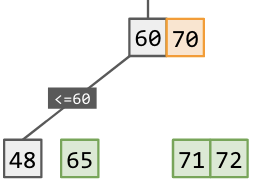
\includegraphics[width=0.35\linewidth]{cs2040s-abtree-split-1.png}
    $\Then$
    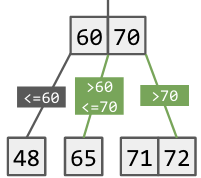
\includegraphics[width=0.28\linewidth]{cs2040s-abtree-split-2.png}
    \item \code{delete(key)} $\Then O(\log n)$
    \begin{itemize}
        \item if the node becomes empty, \code{merge(y, z)} - join it with its left sibling \& replace it with their parent
        \\* 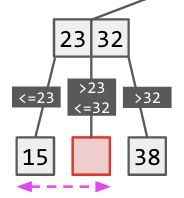
\includegraphics[width=0.25\linewidth]{cs2040s-abtree-delete-1.png}
        $\Then$
        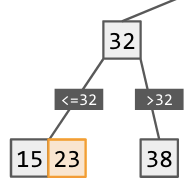
\includegraphics[width=0.3\linewidth]{cs2040s-abtree-delete-2.png}
        \item if the combined nodes exceed max size: \code{share(y, z)} = \code{merge(y, z)} then \code{split()}
    \end{itemize}
\end{itemize}

\textbf{B-Tree (aka $(B, 2B)$-trees)}
\begin{itemize}
    \item possible augmentation: use a linkedList to connect between each level
\end{itemize}

\section{HASH TABLES}
% \begin{itemize}
%     \item disadvantage: no successor/predecessor operation
% \end{itemize}

% \subsection{hashing}
Let the $m$ be the table size; 
let $n$ be the number of items;
let $cost(h)$ be the cost of the hash function

\begin{itemize}
    \item $load(\text{hash table})$, $\alpha = \frac{n}{m}$ 
    \begin{itemize}
        \item = average \& expected number of items per bucket
    \end{itemize}
    \item designing hashing techniques
    \begin{itemize}
        \item \textbf{division method}: $h(k) = k \Mod{m}$ ($m$ is prime)
        \begin{itemize}
            \item don't choose $m = 2^x$
            \item if $k$ and $m$ have common divisor $d$, only $\frac{1}{d}$ of the table will be used
        \end{itemize}
        \item \textbf{multiplication method} - $h(k) = (Ak) \Mod{2^w} \gg (w-r)$ 
        for odd constant $A$ and $m = 2^r$ and $w$ = size of a key in bits
    \end{itemize}
    \item \textbf{simple uniform hashing assumption} 
    \begin{itemize}
        \item \textbf{(1)} every key has an equal probability of being mapped to every bucket; \textbf{(2)} keys are mapped independently
    \end{itemize}
    \item \textbf{uniform hashing assumption} 
    \begin{itemize}
        \item every key is equally likely to be mapped to every permutation, independent of every other key.
        \item NOT fulfilled by linear probing
    \end{itemize}
    \item \textbf{properties of a good hash function}
    \begin{enumerate}
        \item able to enumerate all possible buckets - $h:U \to \{1..m\}$
        \begin{itemize}
            \item for every bucket $j$, $\exists i$ such that $h(key, i) = j$
        \end{itemize}
        \item simple uniform hashing assumption
    \end{enumerate}
\end{itemize}

\subsection{hashCode}
\textbf{rules for the \code{hashCode()} method}
\begin{enumerate}
    \item always returns the same value, if object hasn't changed
    \item if two objects are equal, they return the same hashCode
\end{enumerate}

\textbf{rules for the \code{equals} method}
\begin{itemize}
    \item reflexive, symmetric, transitive for $xRy \iff x.equals(y)$ 
    \item consistent - always returns the same answer
    \item null is null - \code{x.equals(null) => false}
\end{itemize}

\subsection{chaining}
\begin{itemize}
    \item \code{insert(key, value)} - $O(1 + cost(h)) \Then O(1)$
    \begin{itemize}
        \item for $n$ items: expected maximum cost $= O(\log n)$
        \begin{itemize}
            \item $= \Theta(\frac{\log n}{\log(\log(n))})$
        \end{itemize}
    \end{itemize}
    \item \code{search(key)} 
    \begin{itemize}
        \item worst case: $O(n + cost(h)) \Then O(n)$
        \item expected case: $O(\frac{n}{m} + cost(h)) \Then O(1)$
    \end{itemize}
    \item total space: $O(m + n)$
\end{itemize}

\subsection{open addressing - linear probing}
\begin{itemize}
    \item redefined hash function: $h(k, i) = h(k, 1) + i \Mod{m}$
    \item \code{delete(key)}: use a \textit{tombstone value} - DON'T set to \code{null}
    \item \textbf{performance} (assume $\alpha < 1$ and uniform hashing)
    \begin{itemize}
        \item if the table is $\frac{1}{4}$ full, there will be clusters of size $\Theta(\log n)$
        \item expected cost of an operation, $E[\# probes] \leq \frac{1}{1 - \alpha}$
        % \item degrades badly as $\alpha \to 1$
    \end{itemize}
\end{itemize}

\subsubsection{double hashing}
\begin{tightcenter}
    for 2 functions $f, g$, define
    \\* $h(k, i) = f(k) + i \cdot g(k) \Mod m$
\end{tightcenter}
\begin{itemize}
    \item if $g(k)$ is relatively prime to $m$, then $h(k, i)$ hits all buckets
    \begin{itemize}
        \item e.g. for $g(k) = n^k$, $n$ and $m$ should be coprime.
    \end{itemize}
\end{itemize}

\subsection{table size}
assume chaining \& simple uniform hashing
\\ growing the table: $O(m_1 + m_2 + n)$ 
    \begin{tabular}{| c | c | c |}\hline
        \textbf{table growth} & \textbf{resize} & \textbf{insert $n$ items}\\\hline
        \text{increment by 1} & $O(n)$ & $O(n^2)$ \\\hline
        \text{double} & $O(n)$ & $O(n)$, average $O(1)$ \\\hline
        \text{square} & $O(n^2)$ & $O(n)$ \\\hline
    \end{tabular}

\section{SET ADT}
\begin{itemize}
    \item $\checkmark$ speed $\checkmark$ space $\checkmark$ no false negatives $\quad\quad \times$ no ordering 
    % $\quad \times$ may have false positives
\end{itemize}

\subsection{fingerprint hash table}
\begin{itemize}
    \item only stores $m$ bits - does not store the key in a table
    \item $P($no false positives$)$ with SUHA $= (1-\frac{1}{m})^n \approx (\frac{1}{e}^{n/m})$
    \begin{itemize}
        \item i.e. probability of nothing else in the given (same) bucket
        \item for $P($no false positives$) < p$, need $\frac{n}{m} \leq \log(\frac{1}{1-p})$
    \end{itemize}
\end{itemize}

\subsubsection{bloom filter}
\begin{itemize}
    \item 2 hash functions - requires 2 collisions for a false positive
    \item for $k$ hash functions (assume independent slots):
    \begin{itemize}
        \item $P($a given bit is \textbf{0}$) = (1-\frac{1}{m})^{kn} \approx (\frac{1}{e})^{kn/m}$
        \item $P($false positive$) = (1-(\frac{1}{e})^{kn/m})^k$ 
        \item $P($no false positives$) < p$, need $\frac{n}{m} \leq \frac{1}{k}\log(\frac{1}{1-p^{1/k}})$
    \end{itemize}
    \item optimal $k = \frac{m}{n}\ln 2 \quad \then $ error probability $= 2^{-k}$
    \item delete operation: store counter instead of 1 bit
    \item \code{insert, delete, query} $\then O(k)$ 
    \item \code{intersection} (bitwise AND), \code{union} (OR) $\then O(m)$
    \begin{itemize}
        \item gives the same false positives as both 
    \end{itemize}
\end{itemize}


% \section{PROBABILITY THEORY}
% \begin{itemize}
%     \item if an event occurs with probability $p$, the expected number of iterations needed for this event to occur is $\frac{1}{p}$.
%     \item for \textbf{random variables}: expectation is always = probability
%     \item \textbf{linearity of expectation}: $E[A + B] = E[A] + E[B]$
% \end{itemize}

% \section{UNIFORMLY RANDOM PERMUTATION}
% \begin{itemize}
%     \item for an array of $n$ items, every of the $n!$ possible permutations are producible with probability of exactly $\frac{1}{n!}$
%     \begin{itemize}
%         \item the number of outcomes should distribute over each permutation uniformly. (i.e. $\frac{\text{\# of outcomes}}{\text{\# of permutations}} \in \mathbb{N}$)
%     \end{itemize}
%     \item probability of an item remaining in its initial position $= \frac{1}{n}$
%     \item \textbf{KnuthShuffle} $\Then O(n)$ - for (i = n-1..0) \{ swap(i, rand(0, i)) \}
% \end{itemize}

\textbf{KnuthShuffle} $\Then O(n)$ - for (i = n-1..0) \{ swap(i, rand(0, i)) \}

\section{AMORTIZED ANALYSIS}
\begin{tightcenter}
    an operation has \textbf{amortized cost} $T(n)$ if 
    \\* for every integer $k$, the cost of $k$ operations is $\leq kT(n)$.
\end{tightcenter}
\begin{itemize}
    \item \textbf{binary counter ADT}: increment $\then O(1)$
    \item \textbf{hash table resizing}: $O(k)$ for $k$ insertions $\then O(1)$
    \begin{itemize}
        \item search operation: \textit{expected} $O(1)$ (not amortized)
    \end{itemize}
\end{itemize}

\section{GRAPHS}
\begin{itemize}
    % \item \textbf{degree (node)}: number of adjacent edges
    % \item \textbf{degree (graph)}: max. degree of a node
    % \item \textbf{in-/out-degree}: number of incoming/outgoing edges
    % \item \textbf{diameter}: max. shortest path
    % \item even cycles are bipartite!
    \item graph is \textbf{dense} if $\abs{E} = \theta(V^2)$
\end{itemize}
\begin{tabular}{| c | c | c | c | c |}\hline
    adj & \textbf{space} & \textbf{(cycle)} & \textbf{(clique)} & \textbf{use for}\\\hline
    \text{list} & $O(V+E)$ & $O(V)$ & $O(V^2)$ & sparse \\\hline
    \text{matrix} & $O(V^2)$ & $O(V^2)$ & $O(V^2)$ & dense \\\hline
\end{tabular}

\subsection{searching}
\begin{itemize}
    \item \textbf{breadth-first search} $\then O(V+E)$ - queue
    \begin{itemize}
        \item $O(V)$ - every vertex is added exactly once to a frontier
        \item $O(E)$ - every neighbourList is enumerated once
        \item parent edges form a tree \& shortest path from $S$
    \end{itemize}
    \item \textbf{depth-first search} $\then O(V+E)$ - stack
    \begin{itemize}
        \item $O(V)$ - \code{DFSvisit} is called exactly once per node
        \item $O(E)$ - \code{DFSvisit} enumerates each neighbour
        \begin{itemize}
            \item with adjacency matrix: $O(V)$ per node $\then$ total $O(V^2)$
        \end{itemize} 
    \end{itemize}
\end{itemize}

\subsection{shortest paths}
\begin{itemize}
    \item \textbf{Bellman-Ford} $\then O(VE)$
    \begin{itemize}
        \item $\abs{V}$ iterations of relaxing every edge - terminate when an entire sequence of $\abs{E}$ operations have no effect
    \end{itemize}
    \item \textbf{Dijkstra} $\then O((V+E)\log V) = O(E\log V)$
    \begin{itemize}
        \item no negative weight edges!
        \item using a PQ to track the min-estimate node, relax its outgoing edges and add incoming nodes to the PQ
        \item $\abs{V}$ times of \code{insert/deleteMin} ($\log V$ each)
        \item $\abs{E}$ times of \code{relax/decreaseKey} ($\log V$ each)
        \item with fibonacci heap $\then O(E + V \log V)$
    \end{itemize}
    \item \textbf{for DAG} $\then O(E)$ (topo-sort and relax in this order)
    \begin{itemize}
        \item longest path: negate the edges/modify relax function
    \end{itemize}
    \item \textbf{for Trees} $\then O(V)$ (relax each edge in BFS/DFS order)
\end{itemize}

\subsection{topological ordering}
\begin{itemize}
    \item \textbf{post-order DFS} $\then O(V+E)$
    \begin{itemize}
        \item prepend each node from the post-order traversal
    \end{itemize}
    \item \textbf{Kahn's algorithm (lecture vers.)} $\then O(E \log V)$
    \begin{itemize}
        \item add nodes without incoming edges to the topological order
        \item  remove min-degree node from PQ $\then O(V\log V)$
        \item  decreaseKey (in-degree) of its children $\then O(E\log V)$
    \end{itemize}
    \item \textbf{Kahn's algorithm (tutorial vers.)} $\then O(E + V)$
    \begin{itemize}
        \item add nodes with in-degree=0 to a queue; decrement the in-degree of its adjacent nodes. dequeue \& repeat
    \end{itemize}
\end{itemize}

\subsection{spanning trees}
\begin{itemize}
    \item any 2 subtrees of the MSTs are also MSTs
    \item for every cycle, the maximum weight edge is NOT in the MST
    \item for every partition of the nodes, the minimum weight edge across the cut is in the MST
    \begin{itemize}
        \item for every vertex, the minimum outgoing edge is in the MST.
    \end{itemize}
    \item \textbf{Steiner Tree}: (NP-hard) MST containing a given set of nodes
    \begin{enumerate}
        \item calculate the shortest path between any 2 vertices
        \item construct new graph on required nodes
        \item MST the new graph and map edges back to original
    \end{enumerate}
\end{itemize}

\subsection{MST algorithms}
\begin{itemize}
    \item \textbf{Prim's} - $O(E \log V)$
    \begin{itemize}
        \item add the minimum edge across the cut to MST
        \item PQ to store nodes (priority: lowest incoming edge weight)
        \item each vertex: one insert/extractMin $\then O(V \log V)$
        \item each edge: one decreaseKey $\then O(E \log V)$
    \end{itemize}
    \item \textbf{Kruskal's} - $O(E \log V)$
    \begin{itemize}
        \item sort edges by weight, add edges if unconnected
        \item sorting $\then O(E \log E) = O(E \log V)$
        \item each edge: find/union $\then O(\log V)$ using union-find DS
    \end{itemize}
    % \item \textbf{Boruvka's} - $O(E \log V)$
    % \begin{itemize}
    %     \item each node: store a componentId $\then O(V)$
    %     \item one Boruvka step: for each cc, add minimum weight outgoing edge to merge cc's $\then O(V + E)$ dfs/bfs
    %     \begin{itemize}
    %         \item at most $O(\log V)$ Boruvka steps
    %     \end{itemize}
    %     \item update componentIds $\then O(V)$
    % \end{itemize}
    \item \textbf{directed MST with one root} $\then O(E)$
    \begin{itemize}
        \item for every node, add minimum weight \textbf{incoming} edge
    \end{itemize}
\end{itemize}

\section{HEAPS}
\begin{enumerate}
    \item \textbf{heap ordering} - priority[parent] $\geq$ priority[child]
    \item \textbf{complete binary tree} - every level (except last level) is full; all nodes as far left as possible
\end{enumerate}
\begin{itemize}
    \item operations: all $O($max height$) = O(\floor{\log n})$
    \begin{itemize}
        \item \code{insert}: insert as leaf, bubble up to fix ordering
        \item \code{increase/decreaseKey}: bubble up/down larger key
        \item \code{delete}: swap w bottomrightmost in subtree; bubble down
        \begin{itemize}
            \item \code{extractMax}: \code{delete(root)}, bubble down larger key
        \end{itemize} 
    \end{itemize}
    \item heap \textbf{as an array}:
    \begin{itemize}
        \item \code{left(x)} $= 2x + 1$, $\quad$ \code{right(x)} $= 2x + 2$
        \item \code{parent(x)} $= \floor{\frac{x-1}{2}}$
    \end{itemize}
    \item \textbf{HeapSort}: $\then O(n \log n)$ always
    \begin{itemize}
        \item unsorted arr to heap: $O(n)$ (bubble down, low to high)
        \item heap to sorted arr: $O(n \log n)$ (extractMax, swap to back)
    \end{itemize}
\end{itemize}

\section{UNION-FIND}
\begin{itemize}
    \item \textbf{quick-find} - \code{int[] componentId}, flat trees
    \begin{itemize}
        \item $O(1)$ find - check if items have the same componentId
        \item $O(n)$ union - enum all items in array to update id
    \end{itemize}
    \item \textbf{quick-union} - \code{int[] parent}, deeper trees
    \begin{itemize}
        \item $O(n)$ find - check for same root (common parent)
        \item $O(n)$ union - add as a subtree of the root
    \end{itemize}
    \item \textbf{weighted union} - \code{int[] parent}, \code{int[] size}
    \begin{itemize}
        \item $O(\log n)$ find - check for same root (common parent)
        \item $O(\log n)$ union - add as a smaller tree as subtree of root
    \end{itemize}
    \item \textbf{path compression} - set parent of each traversed node to the root - $O(\log n)$ find, $O(\log n)$ union
    \begin{itemize}
        \item a binomial tree remains a binomial tree
    \end{itemize}
    \item \textbf{weighted union + path compression} - for $m$ union/find operations on $n$ objects: $O(n + m\alpha (m, n))$
    \begin{itemize}
        \item $O(\alpha (m, n))$ find, $O(\alpha (m, n))$ union
    \end{itemize}
\end{itemize}
\begin{tightcenter}
    data structures assuming $O(1)$ comparison 
\\* \begin{tabular}{| c | c | c |}\hline
    \textbf{data structure} & \textbf{search} & \textbf{insert}\\\hline
    sorted array & $O(\log n)$ & $O(n)$ \\\hline
    unsorted array & $O(n)$ & $O(1)$ \\\hline
    linked list & $O(n)$ & $O(1)$ \\\hline
    tree (kd/(a, b)/bst) & $O(\log n)$, $O(h)$ & $O(\log n)$, $O(h)$ \\\hline
    trie & $O(L)$ & $O(L)$ \\\hline
    heap & $O(n)$ & $O(\log n)$, $O(h)$ \\\hline
    dictionary & $O(\log n)$ & $O(\log n)$ \\\hline
    symbol table & $O(1)$ & $O(1)$ \\\hline
    chaining & $O(n)$ & $O(1)$ \\\hline
    open addressing & $\frac{1}{1-\alpha} = O(1)$ & $O(1)$ \\\hline
    priority queue & (contains) $O(1)$ & $O(\log n)$ \\\hline
    skip list & $O(\log n)$ & $O(\log n)$ \\\hline
\end{tabular}
% \section{DYNAMIC PROGRAMMING}
% \begin{enumerate}
%     \item \textbf{optimal sub-structure} - optimal solution can be constructed from optimal solutions to smaller sub-problems
%     \begin{itemize}
%         \item greedy algorithms / divide-and-conquer algorithms
%     \end{itemize}
%     \item \textbf{overlapping sub-problems} - can memoize
%     \begin{itemize}
%         \item optimal substructure but no overlapping subproblems = divide-and-conquer
%     \end{itemize}
% \end{enumerate}
% \begin{itemize}
%     \item prize collecting: $\then O(kE)$ or $O(kV^2)$ for k steps
%     \item vertex cover (set of nodes where every edge is adjacent to at least one node) of a tree: $\then O(V)$ or $O(V^2)$
%     \item all pairs shortest path: dijksytra all $\then O(VE\log V)$
%     \item diameter of a graph: SSSP all $\then O(V^2 \log V)$
%     \item floyd warshall $\then O(V^3)$
%     \begin{itemize}
%         \item $S[v, w, P_k]$ = shortest path from $v$ to $w$ only using nodes from set $P$
%         \item $S[v, w, P_8] = \min(S[v, w, P_7], S[v, 8, P_7] + S[8, w, P_7])$
%     \end{itemize}
% \end{itemize}
\begin{align*}
    T(n) &= 2T(\sfrac{n}{2}) + O(n) &\Rightarrow O(n \log n)
    \\ T(n) &= T(\sfrac{n}{2}) + O(n) &\Rightarrow O(n)
    \\ T(n) &= 2T(\sfrac{n}{2}) + O(1) &\Rightarrow O(n)
    \\ T(n) &= T(\sfrac{n}{2}) + O(1) &\Rightarrow O(\log n)
    \\ T(n) &= 2T(n - 1) + O(1) &\Rightarrow O(2^n)
    \\ T(n) &= 2T(\sfrac{n}{2}) + O(n \log n) &\Rightarrow O(n(\log n)^2)
    \\ T(n) &= 2T(\sfrac{n}{4}) + O(1) &\Rightarrow O(\sqrt{n})
    \\ T(n) &= T(n - c) + O(n) &\Rightarrow O(n^2)
    \\ & 3^n \neq O(2^n) \text{ and } 2^{log(n)} = O(n)
\end{align*}
% \textbf{master theorem}
%     \\* $T(n) = aT(\frac{n}{b}) + f(n) \quad a \geq 0, b > 1$
%     $= \begin{cases}
%         \Theta(n^{\log_ba}) & \quad \text{ if } f(n) < n^{\log_ba} \text{ polynomially}
%         \\ \Theta(n^{\log_ba} \log n) & \quad \text{ if } f(n) = n^{\log_ba} 
%         \\ \Theta(f(n)) & \quad \text{ if } f(n) > n^{\log_ba} \text{ polynomially}
%     \end{cases}$
\textbf{orders of growth}
\\* $1 < \log n < \sqrt{n} < n < n \log n < n^2 < 2^n < 2^{2n}$
\\* $\log_a n < n^a < a^n < n! < n^n$ 
\end{tightcenter}

\end{multicols}


\section{FIXXXXXXXXX}
\begin{minipage}{0.5\linewidth}   
    \begin{tightcenter}
        $\begin{array}{| c | c | c | c | c | c |}
            \hline\textbf{sort} & \textbf{best} & \textbf{average} & \textbf{worst} & \textbf{stable?} & \textbf{memory}
    
            \\\hline\text{bubble} & \Omega(n) & O(n^2) & O(n^2) & \checkmark & O(1)
            
            \\\hline\text{selection} & \Omega(n^2) & O(n^2) & O(n^2) & \times & O(1)
            
            \\\hline\text{insertion} & \Omega(n) & O(n^2) & O(n^2) & \checkmark & O(1)
            
            \\\hline\text{merge} & \Omega(n\log n) & O(n\log n) & O(n\log n) & \checkmark & O(n)
            
            \\\hline\text{quick} & \Omega(n\log n) & O(n\log n) & O(n^2) & \times & O(1)

            \\\hline\text{heap} & \Omega(n\log n) & O(n\log n) & O(n\log n) & \times & O(n)
            \\\hline
        \end{array} 
        $\
        \begin{tabular}{| c | c |}
            \multicolumn{2}{c}{sorting invariants}
            \\\hline\textbf{sort} & \textbf{invariant} (after $k$ iterations)
            \\\hline bubble & largest $k$ elements are sorted
            \\\hline selection & smallest $k$ elements are sorted
            \\\hline insertion & first $k$ slots are sorted
            \\\hline merge & given subarray is sorted
            \\\hline quick & partition is in the right position
            \\\hline
        \end{tabular} 
    \end{tightcenter}
    
\end{minipage}

\begin{minipage}{0.48\linewidth}   
    \begin{multicols}{2}
       \section{DYNAMIC PROGRAMMING}
        \begin{enumerate}
            \item \textbf{optimal sub-structure} - optimal solution can be constructed from optimal solutions to smaller sub-problems
            \item \textbf{overlapping sub-problems} - can memoize
            \begin{itemize}
                \item optimal substructure but no overlapping subproblems = divide-and-conquer
            \end{itemize}
        \end{enumerate}
        \begin{itemize}
            \item prize collecting: $\then O(kE)$ or $O(kV^2)$ for k steps
            \item vertex cover (set of nodes where every edge is adjacent to at least one node) of a tree: $\then O(V)$ or $O(V^2)$
            \item diameter of a graph: SSSP all $\then O(V^2 \log V)$
            \item APSP: dijkstra all $\then O(VE\log V)$ or $O(V^2E)$
            \item APSP: floyd warshall $\then O(V^3)$
            \begin{itemize}
                \item $S[v, w, P_k]$ = shortest path from $v$ to $w$ only using nodes from set $P$
                \item ${\scriptstyle S[v, w, P_8] = \min(S[v, w, P_7], S[v, 8, P_7] + S[8, w, P_7])}$
            \end{itemize}
        \end{itemize}
    \end{multicols}
\end{minipage}

\end{document}